\documentclass[10pt, conference, letterpaper]{IEEEtran}
%\IEEEoverridecommandlockouts
% The preceding line is only needed to identify funding in the first footnote. If that is unneeded, please comment it out.
\usepackage{cite}
\usepackage{amsmath,amssymb,amsfonts}
\usepackage{algorithm}
%\usepackage{algorithmic}
\usepackage[noend]{algpseudocode}
\renewcommand{\algorithmicrequire}{\textbf{Input:}}
\renewcommand{\algorithmicensure}{\textbf{Output:}}
%\usepackage{definition}
\usepackage{graphicx}
\ifCLASSOPTIONcompsoc
	\usepackage[caption=false, font=normalsize, labelfont=sf, textfont=sf]{subfig}
\else
	\usepackage[caption=false, font=footnotesize]{subfig}
\fi
%\usepackage{amssymb}
\usepackage{textcomp}
\usepackage{xcolor}
\usepackage{bm}
\newtheorem{definition}{Definition}
\def\BibTeX{{\rm B\kern-.05em{\sc i\kern-.025em b}\kern-.08em
    T\kern-.1667em\lower.7ex\hbox{E}\kern-.125emX}}
    
\newcommand{\cb}{\textcolor[rgb]{1.00,0.00,0.00}}
    
    
\begin{document}

\title{Efficient Coflow Scheduling of Multi-stage Jobs with Isolation Guarantee}

\author{Zifan Liu, Haipeng Dai, Bingchuan Tian, Wajid Rafique, and Wanchun Dou\\
State Key Laboratory for Novel Software Technology, Nanjing University, Nanjing, Jiangsu 210023, China\\
\{zifanliu, bctian, rafiqwajid\}@smail.nju.edu.cn, \{haipengdai, douwc\}@nju.edu.cn}

\maketitle

\begin{abstract}
Coflow scheduling is critical for data-parallel computing performance in datacenters. Performance and isolation guarantee have become two major objectives for coflow scheduling. However, in the context of multi-stage jobs, existing coflow scheduling frameworks only focus on minimizing the average job completion time (JCT) while overlooking the isolation guarantee. To address this problem, in this paper we propose the first coflow scheduling scheme that %to achieve near-optimal performance with attainable isolation guarantee. To the best of our knowledge, this is the first work 
aims to achieve both objectives.
%
We show that our scheduler outperforms existing alternatives significantly in minimizing average JCT while guaranteeing that no job will be delayed beyond a constant time than its JCT in a fair scheme. Our evaluation results show that our scheduler reduces the average JCT by at least 86\% compared with state-of-the-art schedulers.
\end{abstract}

\begin{IEEEkeywords}
datacenter network, coflow scheduler, multi-stage jobs
\end{IEEEkeywords}

\section{Introduction}
Data-parallel frameworks, such as MapReduce\cite{MapReduce}, Hadoop\cite{Hadoop} and Spark\cite{Spark}, are widely deployed in modern datacenters. Various distributed computing jobs (\emph{e.g.}, data mining or querying) are run by these frameworks, where intermediate data is transferred between a group of machines. For example, a MapReduce job distributes mapper tasks and reducer tasks on two sets of machines (not necessarily be disjoint) determined by a master process. Each mapper task reads input data from local disks or networks and produces intermediate key/value pairs. Each reducer task accepts a set of keys and values for those keys, merges values together, and writes the final output data to local files. The intermediate data needs to be transferred from mapper machines to reducer machines and such process is called as a \emph{shuffle} phase. These flows are reported to may account for over 50\% of job completion time, which has a significant impact on job performance.

The \emph{coflow} abstraction was proposed to help improve shuffle performance. A coflow means a collection of parallel flows\cite{coflow}. In the MapReduce case, flows in one \emph{shuffle} phase are termed a coflow. %Traditional network performance metrics, such as average flow-completion-time (FCT), neglect application-level communication pattern of data-parallel jobs.
Not until all parallel flows have finished transmission will the MapReduce shuffle phase complete, thus only the slowest flow %(not the average FCT)
in a coflow determines the start time of reducer tasks. Hence, to reduce the coflow-completion-time (CCT), the optimization scheduling framework should schedule flows in coflow level rather than flow level. Many recent works focus on achieving optimal performance, \emph{e.g.}, minimizing average coflow-completion-time\cite{varys,aalo,coda,barrat,stream}. In the meantime, many network schedulers settle for offering optimal isolation among coflows\cite{HUG,DRF,faircloud,fair}. These schedulers guarantee fair bandwidth sharing for all coflows so that the predictable CCTs can be provided.

However, achieving both the above targets simultaneously is challenging in the multi-stage job scenario. First, for jobs containing only one shuffle phase, since there is only one coflow in a job, minimizing average CCT usually leads to faster jobs. However, for the multi-stage jobs, minimizing average CCT does not always result in faster jobs because the dependencies in a job should be considered. Tian \emph{et al.}\cite{bingchuan} took the first step on minimizing multi-stage job-completion-time (JCT), but did not give attention to the isolation between jobs. Second, schedulers providing optimal isolation usually allocate fair share network bandwidth to all coflows. %, giving the completion of coflows predictable CCTs
However, fair scheduling may fail short in poor coflow performance (\emph{i.e.}, minimizing average CCT)\cite{HUG}. Performance and fairness have been considered as conflict objectives for long time. Wang \emph{et al.}\cite{utopia} attempted to achieve both objectives, but they did not consider multi-stage jobs.

In the context of multi-stage jobs, we say that coflow $C_2$ is dependent on another coflow $C_1$ if the computation stage of $C_1$ is the producer of $C_2$. There are two types of dependencies: \emph{Start-After} and \emph{Finishes-Before}. \emph{Start-After} indicates the entity of explicit barriers\cite{Hadoop}, which means coflow $C_2$ cannot start before coflow $C_1$ completes. \emph{Finishes-Before} means coflow $C_2$ can coexist with coflow $C_1$ but cannot complete until $C_1$ has completed, which is common for the pipeline of continuing stages\cite{dryad}. We focus on scheduling jobs with \emph{Start-After} type dependencies in the rest parts of this paper, and leave the \emph{Finishes-Before} dependencies to future work.

In this paper, we aim to address the challenge of achieving both of optimal performance and isolation guarantee in the context of multi-stage jobs. Generally, we make the following major contributions.

First, to the best of our knowledge, this is the first work for the studies: \emph{how to schedule dependent coflows of multi-stage jobs to provide long-term isolation guarantee while minimizing the average JCT} (Section~\ref{related}).

Second, We present a formal mathematical formulation for this probelm (Section~\ref{model}) and propose a novel coflow scheduler for multi-stage jobs (Section~\ref{algorithm}). The key idea of our approach is to allocate bandwidth to coflows in the priority order depending on their completion times under fair schedulers (\emph{e.g.}, DRF\cite{DRF} or HUG\cite{HUG}). We find this idea can lead to the best of both objectives for the following two reasons. First, since fair schedulers offer coflows the same progress, small coflows seem to complete earlier than large ones. % Like performance optimal schedulers, such as Varys\cite{varys}, small coflows have higher priority than large ones to minimize the average CCT.
Second, the isolation service can only be observed by applications when coflows complete. Our approach tends to complete coflows earlier than they would have for a fair scheduler, thus a \emph{long-term isolation guarantee} is provided to applications. %To deal with the multi-stage jobs, we will set the priorities in two levels: \emph{inter-job priority} and \emph{intra-job priority}. \emph{Inter-job priority} means the faster a job completes in a fair scheduler, the higher priority it is given. \emph{Intra-job priority} means within a job, earlier completed coflows in a fair scheduler have higher priorities than the later ones.

Finally, we evaluate the performance of our scheduler by comparing it with three state-of-the-art schedulers: HUG\cite{HUG}, Aalo\cite{aalo}, and Utopia\cite{utopia}. Results indicate that our scheduler can provide guaranteed isolation between jobs and the job slowdown can be reduced by at least 86\% compared with the state-of-the-art schedulers (Section~\ref{evaluation}).

\section{Related Work}\label{related}
Existing works mostly focus on scheduling coflows in single-stage jobs. These schedulers usually settle on one goal (performance or isolation) as the primary objective, while ignoring or treating the other one as a secondary objective. We will discuss these schedulers in the aspects of primary objectives.

\noindent\textbf{Performance-optimal:} Many schedulers focus on minimizing average CCT. Orchestra\cite{orchestra} first presents the coflow abstraction and shows that even a simple FIFO algorithm can significantly improve coflow performance. Varys\cite{varys} uses the \emph{smallest-effective-bottleneck-first} (SEBF) heuristic to sort coflows and the \emph{minimum-allocation-for-desired- duration} (MADD) heuristic to preferentially allocate least bandwidth to coflows for minimizing average CCT and deadline missing rate. CODA\cite{coda} aims at scheduling information-agnostic coflows by automatically collecting coflow information. Barrat\cite{barrat} and Stream\cite{stream} focus on decentralized coflow scheduling. These schedulers cannot handle the dependencies and minimize average JCT for multi-stage jobs. To the best of our knowledge, only \cite{aalo} and \cite{bingchuan} consider multi-stage jobs and attempt to minimize average JCT. 
%The only schedulers that take multi-stage jobs for concern are Aalo\cite{aalo} and an approximation algorithm presented by Tian \emph{et al.}\cite{bingchuan}. %Aalo uses only one short section to discuss a simple heuristic for minimizing average JCT. %Tian's algorithm cannot guarantee isolation between jobs.

\noindent\textbf{Isolation-optimal:} There are also some schedulers aiming at providing isolation guarantee to coflows. HUG\cite{HUG} seeks Dominant Resource Fairness (DRF)\cite{DRF} to allocate fair share of bandwidth to coflows. Chen \emph{et al.}\cite{optimizing} assumed that coflows have respective utility fuctions and developed an approximation algorithm to address the obtained optimal max-min fairness problem. NC-DRF\cite{fair} provides isolation guarantee to non-clairvoyant coflows with the coflow correlation information. These schedulers fall short in longer average CCT and cannot provide near-optimal performance.

\noindent\textbf{Both two objectives:} Coflex\cite{coflex} and Utopia\cite{utopia} are the only two schedulers that consider both the two objectives with same importance. Coflex is proposed as a middle ground between Varys and HUG, which navigates the tradeoff space between performance and isolation with an elastic \emph{fairness knob} in the range of 0 to 1. However, such knob is hard to be determined in real-world systems. Utopia uses super-coflow scheduling to provide isolation guarantee with near-optimal performance, but cannot handle the multi-stage jobs.

\section{Model and Objective}\label{model}
In this section, we firstly introduce the model of datacenter networks and coflow, and then discuss two objectives. To simplify the discussion, key terms used in our model are summarized in Table~1.
\begin{table}
\caption{Key Terms and Descriptions}
\begin{center}
\begin{tabular}{|r|l|}
\hline
Terms & Description\\
\hline
$M$ & Number of total jobs\\
\hline
$N$ & Number of total coflows\\
\hline
$K$ & Number of machines\\
\hline
$F_i = \left\langle f_i^1,\dots,f_i^{2K}\right\rangle$ & Demand vector of coflow-$i$\\
\hline
$d_i = \left\langle d_i^1,\dots,d_i^{2K}\right\rangle$ & Correlation vector of coflow-$i$\\
\hline
$c_i=\left\langle c_i^1,\dots,c_i^{2K}\right\rangle$ & Bandwidth allocation of coflow-$i$\\
\hline
$\overline{f_i}=\max_{k} f_i^k$ & Bottleneck demand of coflow-$i$\\
\hline
$P_i$ & Progress of coflow-$i$\\
\hline
$\Gamma_i$ & Progress of job-$i$\\
\hline
$T_i$ & JCT of job-$i$\\
\hline
$T_i^*$ & JCT of job-$i$ under a fair scheduler\\
\hline
\end{tabular}
\end{center}
\end{table}

\subsection{Model}
Given the full bisection bandwidth, which has been well developed in modern datacenter\cite{jupiter}, we treat the datacenter network as a big non-blocking switch connecting $K$ machines. Each machine has one uplink port and one downlink port, thus the whole fabric has $2K$ ports. In this simplified model, the ports are the only congestion points. Therefore, we focus sorely on bandwidth of each port. In our analysis, all links are assumed to be of equal capacity that is normalized to one.

The coflow abstraction presents the communication demand between stages of parallel computing frameworks. A coflow is composed of a collection of flows across a group of machines sharing a common performance requirement. The completion time of the latest flow defines the completion time of this coflow. In many data-parallel frameworks like MapReduce/Hadoop, the job and coflow properties, such as source, destination, amount of data transferred of each flow, coflow dependencies are known as a priori\cite{varys, aalo, bingchuan}. In this paper, we assume that all jobs are released at time 0 and all coflows with no dependencies start at time 0 too.

Specifically, the coflow \emph{demand vector}, say $F_i = \left\langle f_i^1,\dots,f_i^{2K}\right\rangle$, captures the data demand of coflow-$i$, where $f_i^k$ denotes the amount of data transferred on port $k$. Additionally, $f_i^{hl}$ denotes a flow transferring data from port $h$ to port $l$. Among all flows in coflow-$i$, we name the port with the largest traffic as bottleneck port. Let the data demand on this port be the \emph{bottleneck demand}, defined as $\overline{f}_i=\max_{k} f_i^k$. To simplify our analysis, the \emph{correlation vector}, say $d_i = \left\langle d_i^1,\dots,d_i^{2K}\right\rangle$, is engaged to describe the demand correlation across ports, where $d_i^k$ is the normalized data demand on port $k$ by the bottleneck demand, \emph{i.e.}, $d_i^k = f_i^k/\overline{f}_i$. This vector indicates that for every byte coflow-$i$ sent on bottleneck port, at least $d_i^k$ bytes should be transferred on port $k$.

Coflows have elastic bandwidth demands on multiple ports, which means that the \emph{bandwidth allocation vector}, say $c_i=\left\langle c_i^1,\dots,c_i^{2K}\right\rangle$, of coflow-$i$, where $c_i^k$ is the bandwidth share on port $k$, is not necessarily in the same ratio of demand vector $d_i$. Given the bandwidth allocation vector $c_i$ for each coflow-$i$ calculated by coflow scheduler given the demand vectors, the coflow progress is restricted by the worst-case port. Formally, \emph{progress} of coflow-$i$ is defined as the minimum demand-normalized rate allocation across ports, \emph{i.e.},
 \begin{equation}
 	P_i = \min\limits_{i:d_i^k>0}\frac{c_i^k}{d_i^k}.
 \end{equation}
 Intuitively, progress of coflow-$i$ means the smallest demand satisfaction ratio across all ports, which determines the CCT of coflow-$i$.

Assume that a multi-stage job-$m$ has $N$ active coflows, \emph{i.e.}, $\left\{F_{m,1},\dots,F_{m,N}\right\}$. Given the bottleneck demand $\left\{\overline{f}_{m,1},\dots,\overline{f}_{m,N}\right\}$ and progress $\left\{P_{m,1},\dots,P_{m,N}\right\}$ of each coflow, the progress of job-$m$ can be computed as the weighted average progress of active coflows in job-$m$, \emph{i.e.},
\begin{equation}
	\Gamma_m = \frac{\sum_{n=1}^N \overline{f}_{m,n}P_{m,n}}{\sum_{n=1}^N \overline{f}_{m,n}},
\end{equation}
where $\overline{f}_{m,n}$ is the weight of coflow $F_{m,n}$. Similarly, progress of job-$m$ indicates the collectivity smallest demand satisfaction ratio of all coflows belonging to it, which has significant effect on the JCT of job-$m$.

\subsection{Objective}
%In common consensus\cite{coflow, coflex, utopia}, a coflow scheduler focuses primarily on two objectives, average CCT and isolation guarantee. 
For the multi-stage coflow  scheduling problem, we are concerned with the average JCT and isolation guarantee.

\begin{enumerate}
	\item \emph{Average JCT}: To speed up data-parallel application completion time, as many jobs as possible should be finished in their fastest possible ways. Therefore, minimizing the average JCT is a critical objective for an efficient coflow scheduler.
	\item \emph{Isolation Guarantee}: In a shared datacenter network, all tenants expect \emph{performance isolation guarantees}. Existing work has defined such guarantee as the \emph{minimum progress} across coflows\cite{HUG}, \emph{i.e.}, $\max_i P_i$. For multi-stage jobs, we define the isolation guarantee as the minimum progress across active jobs, \emph{i.e.}, $\max_m \Gamma_m$. To optimize the isolation guarantee, a coflow scheduler should look for an allocation to maximize the minimum progress.
\end{enumerate}

However, on the application level, the effect of isolation guarantee cannot be perceived until the job is finished. If we take the fair scheme (\emph{e.g.}, DRF\cite{DRF} or HUG\cite{HUG}) as a baseline, as long as an application observes that its jobs finish no later than the time point at which they would have finished in the baseline algorithm, the isolation guarantee is provided in long run. Thus, we introduce the job \emph{long-term isolation guarantee} to our model.

\textbf{Definition 1 (Long-term Isolation Guarantee):} Consider a multi-stage job-$i$, let $T_i$ be its JCT by coflow scheduler $S$. $T_i^*$ is its JCT by a fair scheduler that enforces a minimum instantaneous progress of all active coflows. We call the scheduler $S$ provides the job long-term isolation guarantee if all jobs complete no later than $T_i^* + D$, where $D$ is a constant delay, \emph{i.e.},
\begin{equation}
	T_i \leq T_i^* + D.
\end{equation}

In this paper, our objective is to gain the best performance regarding both targets in a long run, which is formalized as
\begin{equation}
	\begin{aligned}
		\text{minimize} & & &\sum\limits_{i}T_i,\\
		\text{s.t.} & & &T_i \leq T_i^* + D \text{, for all job-}i.\\
	\end{aligned}
\end{equation}

\section{Algorithm and Analysis}\label{algorithm}
In this section, we design a coflow scheduling algorithm of multi-stage jobs with isolation guarantee. We first elaborate on how to sort coflows based on their priorities. Then, we propose our bandwidth allocation algorithm.

\subsection{Coflow Sorting}
Before we allocate bandwidth to coflows, the priority of each coflow should be determined. Suppose all coflows are scheduled by the fair scheduler DRF, which enforces the equal progress across coflows\cite{DRF,HUG}. Based on the completion time of each coflow under such scheduling, we can obtain a priority order for all coflows. If a coflow completes earlier in DRF scheduling, it has a higher priority than the others.

However, directly performing DRF is not suitable in the context of multi-stage jobs, because some coflows that have dependencies are not released at the start. At first, we can only calculate the completion time of each coflow in $F'$ with no dependencies, which are released at time 0. Then, the minimum progress of these coflows $P^* = \min_iP'_i$ is produced, where $P'_i$ is the progress of $F'_i$. Note that in popular parallel frameworks, the numbers of coflows in different stages are similar \cite{Spark,coflowsurvey}. We assume that $P^*$ keeps unchanged across stages, then the completion time of coflow $F_i \notin F'$ is estimated as $t_i = P^*\overline{f_i}$.

We assume that the job $J_i$ is the $i$-th job to complete data transferring, \emph{i.e.}, when $J_i$ completes, $J_1,\dots,J_{i-1}$ have already completed. Let $(F_{i,1},\dots,F_{i,N_i})$ be the coflows constituting job $J_i$ in the topological order.

Besides, the completion time of single coflow is not necessarily the priority of the job containing it. In multi-stage jobs, coflow pipelines are developed using directed acyclic graph (DAG) pattern to show the dependencies between coflows. In job-$i$, we set the weights of coflows in DAG as their completion time. Then, we can get the \emph{estimate completion time} of coflow-$j$ $F_{i,j}$ as the maximum total weight along DAG edges from roots to coflow-$j$. A coflow with shorter estimate completion time has a higher priority. Additionally, the estimate completion time of job-$m$ is the maximum estimate completion time of all coflows it contains. Similarly, if a job completes earlier, it has a higher priority. Within a job, the priority order of coflows is the ascending order of estimate completion time. Therefore we get a prioritized queue of all coflows $\mathbf{F} = (F_{1,1},\dots,F_{1,N_1},\dots,F_{M,1},\dots,F_{M,N_M})$. The entire procedure is summarized in Algorithm~1.

\begin{algorithm}
	\caption{Coflow Sorting Algorithm}
	\begin{algorithmic}[1]
		\Require Data demand set of all coflows $F$ and the job set $J$.
		\Ensure An ordered queue of all coflows $\mathbf{F}$.
		\State Sort $F$ in the topological order of DAG.
		\State $F' \gets $ coflows have no dependencies in $F$.
		\State $P^* \gets$ the minimum progress of $F'$ under DRF.
		\For{$i = 1 \to \left|F\right|$}
			\If{$F_i \in F'$}
				\State $t_i \gets$ the completion time of $F_i$ under DRF.
			\Else
				\State $t_i \gets P^*\overline{f}_i$.
			\EndIf
			\If{$F_i \text{ has dependencies }$}
				\State $t_i \gets t_i + \max{\{t_j|F_i \text{ depends on } F_j\}}$.
			\EndIf
		\EndFor
		\State $T_m \gets$ the maximum total time along DAG edges of $J_m$.
		\State Sort $J$ in the ascending order of $T$.
		\State Initialize $\mathbf{F}$ as an empty queue.
		\For{$m = 1 \to \left|J\right|$}
			\State $\overline{F}_m \gets$ coflows of $J_m$ in the ascending order of $t$.
			\State $\mathbf{F} \gets \mathbf{F} + \overline{F}_m$.
		\EndFor
	\end{algorithmic}
\end{algorithm}

\subsection{Bandwidth Allocation}
After obtaining the prioritized queue of coflows, we can allocate bandwidth to the active coflows one by one. Specifically, we introduce the \emph{super-coflow} conception which was proposed in \cite{utopia} for our solution.

\noindent \textbf{Super-coflow.} Given a queue of coflows $\mathbf{F}$, the super-coflow $S_i$ is defined as the sequential aggregation of the first $i$ coflows $F_1,\cdots,F_i$. Formally, the demand vector $D_i = \langle D_i^1,\dots,D_i^{2K} \rangle$ of $S_i$ is the accumulation of the first $i$ coflows, \emph{i.e.}, $D_i = \sum_{j=1}^if_j$. Super-coflow $S_1$ trivially degrades into coflow $F_1$ as a special case.

In previous works, coflows are mostly scheduled individually. We take as an example the minimum-allocation-for-desired-duration (MADD) algorithm, which is a common approach for sequential coflow bandwidth allocation \cite{varys, orchestra}. In MADD, the least amount of bandwidth was allocated to a coflow to obtain the maximum possible progress. Let $R_k$ be the remaining bandwidth on port $k$ and $d_i=\langle d_i^1,\dots,d_i^{2K}\rangle$ be the correlation vector of coflow-$i$. Thus, the maximum possible progress $P'$ of coflow-$i$ can be calculated as
\begin{equation}
	P' = \min_{1\leq k \leq 2K}\frac{R_k}{d_i^k}.
\end{equation}
To acquiring the maximum possible progress, the bandwidth allocation of coflow-$i$ on port $k$ is at least $P'd_i^k$. In MADD, the allocation is exactly $P'd_i^k$.

However, MADD may lead to the priority inversion problem. If a coflow is not able to get any progress, then it gets no bandwidth, even if allocating it some bandwidth will accelerate its completion. To further explain priority inversion, we consider a motivating example in Fig.~\ref{motivative}. Three coflows ($A$, $B$, and $C$) transfer data through three ports whose bandwidths are uniformed to be 1. Coflow-$A$, coflow-$B$, and coflow-$C$ have demand vectors $F_A=\langle 3,0,0\rangle$, $F_B=\langle 1,4,2\rangle$, and $F_C=\langle 0,6,5\rangle$, respectively. Since coflow-$A$ has the smallest bottleneck demand 3, it has the highest priority, followed by coflow-$B$. The priority order of the three coflows is $A > B > C$. Fig.~\ref{motivative}(a) shows the bandwidth allocation for the MADD scheme. At time 0, coflow-$B$ cannot get any bandwidth on port 1, \emph{i.e.}, it cannot get any progress, so no bandwidth is allocated to coflow-$B$ but to coflow-$C$ on ports 2 and 3. Coflow-$B$ is preempted by coflow-$C$, whereas in an optimal scheme, coflow-$B$ still should gain bandwidth on ports 2 and 3 as shown in Fig.~\ref{motivative}(b).

\begin{figure}[!t]
	\centering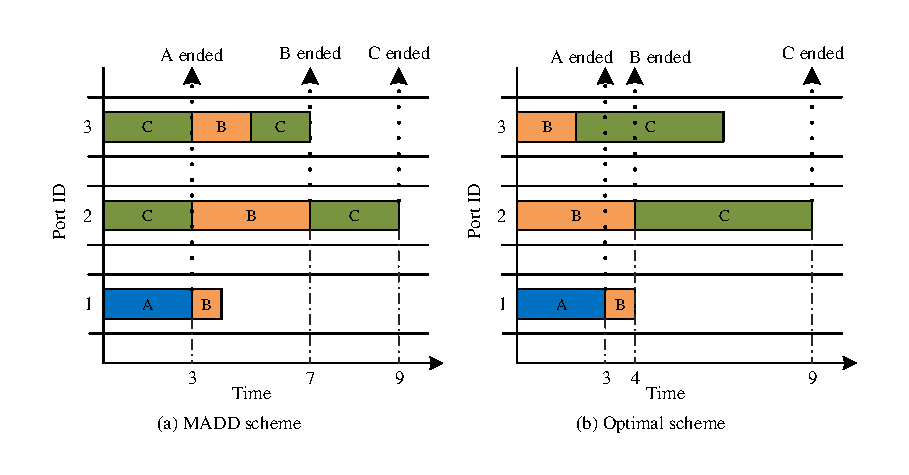
\includegraphics[width=1.03\linewidth]{motivative.eps}
	\caption{Priority inversion in MADD. Coflows transfer data through three ports whose bandwidths are uniformed to be 1. Three coflows have demand vectors $F_A=\langle 3,0,0\rangle$, $F_B=\langle 1,4,2\rangle$, and $F_C=\langle 0,6,5\rangle$. The priority order of the three coflows is $A > B > C$.}\label{motivative}
\end{figure}


On the contrary, our super-coflow conception eliminates the priority inversion situation as much as possible. When computing the bandwidth allocation, coflow $F_i$ is justified if it contributes to super-coflow $S_i$. As long as $F_i$ affects the progress of $S_i$, a bandwidth allocation to $F_i$ is always guaranteed, even when it gains no progress alone, which easily triggers a priority inversion.

Assume that the active coflow priority queue is $F'=(F'_1,\dots,F'_{N'})$. Our bandwidth allocation algorithm runs in turns. In the $i$-th turn, we will allocate the least bandwidth to $F'_i$, while the allocations of earlier turns stay unchanged,  in order to achieve the minimum possible completion time of $S_i$. To easily describe our algorithm, we next focus on the bandwidth allocation of $F'_i$.

To achieve the minimum possible completion time of $S_i$, we first calculate the bottleneck data demand of $S_i$, \emph{i.e.},
\begin{equation}
	\overline{D}_i = \max_{1\leq k\leq 2K}D_i^k.
\end{equation}
Let $D_i^{hl}$ be the data amount transferred from port $h$ to port $l$ in $S_i$. Then, at least $D_i^{hl}/\overline{D}_i$ bandwidth should be allocated for the flows between port $h$ and port $l$. Note that the first $i-1$ coflows have received some bandwidth in the earlier turns. We denote the bandwidth received by flow $f_k^{hl}$ in coflow-$k$ as $u_k^{hl}$ for $k < i$, thus we can distribute at most $(D_i^{hl}/\overline{D}_i - \sum_{k=1}^{i-1}u_k^{hl})^+$ bandwidth to $f_i^{hl}$, where $(x)^+=\max(0,x)$. Given the remaining bandwidth $R_h$ on port $h$ and $R_l$ on port $l$, which limit the actual bandwidth available for $f_i^{hl}$, we finally get $u_i^{hl}$ as
\begin{equation}
	u_i^{hl} = \min[(D_i^{hl}/\overline{D}_i - \sum_{k=1}^{i-1}u_k^{hl})^+,R_h,R_l].
\end{equation}
After that, the remaining bandwidth on these two ports are updated. When all turns have finished, unused bandwidth is distributed to coflows. For each ingress port $h$, remaining bandwidth $R_h$ is distributed to corresponding flows according to ratio of their current received bandwidth $u_i^{hl}$, restricted by the corresponding egress port $l$. We summarize the whole procedure as $\mathsf{SuperflowAllocation}(F)$ in Algorithm~2.
%\begin{theorem}[Super-coflow]
%	Given a queue of coflows $\mathbf{F}$, the super-coflow $S_i$ is defined as the aggregation of the first $i$ coflows. Formally, the demand vector $D_i = \langle D_1,\dots,D_{2K} \rangle$ of $S_i$
%\end{theorem}
%\begin{itemize}
%	\item \textbf{Super-coflow}
%\end{itemize}

\begin{algorithm}
	\caption{Bandwidth Allocation Algorithm}
	\begin{algorithmic}[1]
		\Procedure{SuperflowAllocation}{Coflows $F$}
			\State Initialize unused bandwidth $R_k \gets 1$ on port-$k$
			\For{$i = 1 \to \left|F\right|$}
				\State Assemble demands $D_i = \sum_{k=1}^if_k$.
				\State $\overline{D}_i \gets \max_kD_i^k$.
				\ForAll{flow $f_i^{hl} \in F_i$}
					\State $u_i^{hl} \gets \min[(D_i^{hl}/\overline{D}_i - \sum_{k=1}^{i-1}u_k^{hl})^+, R_h,R_l]$.
					\State $R_h \gets R_h - u_i^{hl}$.
					\State $R_l \gets R_l - u_i^{hl}$.
				\EndFor
			\EndFor
			\State Allocate remaining bandwidth to all coflows.% in the order of $F$ by FIFO.
		\EndProcedure
		\Procedure{BandwidthAllocation}{Coflows $F$}
			\State $\mathbf{F} \gets$ sorted $F$ by Algorithm~1.
			\State Initialize active coflows $F' \gets \emptyset$.
			\While{True}
				\State $F' \gets$ released coflows in the order of $\mathbf{F}$.
				\If{$F'$ is changed}
					\State Update remaining transfer demand of $F'$.
					\State SuperflowAllocation($F'$).
				\EndIf
				\If{$F' == \emptyset$}
					\State \textbf{break}.
				\EndIf
			\EndWhile
		\EndProcedure
	\end{algorithmic}
\end{algorithm}

When an old coflow is finished or a new coflow is released, the active coflow set $F'$ is changed and the bandwidth allocations will be rescheduled. All the active coflows are sorted as the order we get by Algorithm~1 to maintain the priorities of all jobs through our scheduling. The main procedure is summarized as $\mathsf{BandwidthAllocation}(F)$ in Algorithm~2.

\subsection{Long-term Isolation Guarantee}
Our algorithm provides the job long-term isolation guarantee of Definition~1. For each job-$i$, the completion time $T_i$ is guaranteed not to exceed a constant time over its completion time in DRF. Thus, we have the following theorem:

\textbf{Theorem 1 (Long-term Isolation Guarantee):} Assume that jobs $J$ are released at time 0. For each job $J_i \in J$, let $T_i$ be the JCT of $J_i$ in Algorithm~2, and let $T_i^*$ be the completion time of $J_i$ in DRF. The completion time delay is bounded as
\begin{equation}
	T_i \leq T^* + \overline{f}_i.
\end{equation}

\begin{IEEEproof}
To simplify our proof, we abbreviate $F_{i,N_i}$ and $S_{i,N_i}$ to $F_i$ and $S_i$ through this proof and let $F(i)$ be the coflows before $F_i$ in our priority order. Since $F_i$ is the last completed coflow of $J_i$, the JCT of $J_i$ (\emph{i.e.}, $T_i$) equals to the completion time of $F_i$. Additionally, we let $F_0(i)$ be the coflows that has shorter estimate completion time than $F_i$, \emph{i.e.}, coflows in $F_0(i)$ are the ones finished before $F_i$ in DRF. We have $F(i) \subseteq F_0(i)$ because all coflows in $\{J_1,\dots,J_i\}$ except $F_i$ have shorter estimate completion time than $F_i$. To discuss $T_i$, we consider the following two cases.

\emph{Case~1.} The bottleneck port of super-coflow $S_i$ is kept using full bandwidth during the data transmission. In this case, the completion time of $S_i$ is simply the time of transferring data on bottleneck port, \emph{i.e.}, $\overline{D}_i$. When $S_i$ completes, $F_i$ must have completed. Therefore, we have $T_i \leq \overline{D}_i$. Then, we turn to DRF. According to our algorithm, all jobs are sorted by their JCT in DRF. When $J_i$ completes, previous $i-1$ jobs $J_1,\dots,J_{i-1}$ must have all completed, so does $S_i$. Note that $\overline{D}_i$ is the minimum possible completion time of $S_i$, \emph{i.e.}, $\overline{D}_i \leq T_i^*$, thus we finally have
\begin{equation}\label{case1}
	T_i \leq \overline{D}_i \leq T_i^*.
\end{equation}

\emph{Case~2.} The bottleneck port of super-coflow $S_i$ is not fully used at some time during the data transmission. Recall that the bandwidth allocation on bottleneck port is constrained by the available bandwidth on the coupled ports due to Line 7 in Algorithm~2. In particular, we define port $k$ as a coupled port of port $l$ if there are flows in $S_i$ transferring data between these two ports but getting less bandwidth allocation than $D_i^{kl}/\overline{D}_i$. Let $B_i$ be the bottleneck port of $S_i$ and let $C(B_i)$ be the set of coupled ports of $B_i$. Additionally, let $C_0(B_i)$ be the ports that have data transmission with $B_i$ in $S_i$.

Let $t_B$ be the time when port $B_i$ starts to get full bandwidth allocation until the completion of $S_i$. Specifically, let $t_k$ be the time when port $k$$\in$$C(B_i)$ finishes data transmission of all the coflows in $F(i)$. In our algorithm, the lacking of bandwidth utilization on $B_i$ can only occur when bandwidth of each port in $C(B_i)$ is fully used, otherwise our algorithm will attempt to allocate the spare bandwidth to a flow between such coupled port and $B_i$. Therefore, we have
\begin{equation}
	t_B \leq \max_{k \in C(B_i)} t_k.
\end{equation}

Since the bandwidth allocation of each port varies throughout the data transmission because of completions of coflows, we denote $a_i^{kl}(t)$ and $b_i^{kl}(t)$ as the expected and actual bandwidth allocation of the flows  of $S_i$ transferring between port $k$ and port $l$ at time $t$. In particular,
\begin{align}
	\label{actual} a_i^{kl}(t) &= D_i^{kl}(t)/\overline{D}_i(t);\\
	b_i^{kl}(t) &= u_i^{kl}(t) + \sum_{j\in F(i)}u_j^{kl}(t).
\end{align}

Note that during the transmission of $S_i$, the actual bandwidth allocation on some ports may continue being less than its expected bandwidth when $S_i$  is running alone under DRF. In some extreme situations, the bottleneck port of $S_i$ may change from $B_i$ to another port $k$ if port $k$ keeps getting less bandwidth allocation than expected, which we call the bottleneck port of $S_i$ \emph{shifts}. To bound our JCT of $J_i$, we next discuss two sub-cases, differentiated by whether the bottleneck port of $S_i$ shifts.

\emph{Sub-Case~1.} The bottleneck port $B_i$ of $S_i$ does not \emph{shift} during the data transmission. In the worst case, bottleneck port $B_i$ can only get full bandwidth allocation when all previous coflows finish their data transmissions on the coupled ports of $B_i$, which means $t_B = \max_{k\in C(B_i)}t_k$. We have the JCT constraint of $J_i$ as
\begin{equation}\label{sc:1}
	T_i \leq \overline{D}_i + \sum_{k\in C_0(B_i)}\int_0^{t_k}(a_i^{kB_i}(t)-b_i^{kB_i}(t))dt.
\end{equation}
Since $S_i$ is the aggregation of $F(i)$ and $F_i$, we can split $\overline{D}_i$ into two parts as
\begin{equation}\label{sc:2}
	\overline{D}_i = f_i^{B_i} + \mathbf{D}_i^{B_i},
\end{equation}
where $f_i^{B_i}$ is the data demand of $F_i$ on port $B_i$ and $\mathbf{D}_i^{B_i}$ is the sum of data demands of coflows in $F(i)$ on $B_i$. Thus, we have
\begin{equation}\label{sc:3}
	\mathbf{D}_i^{B_i} = \sum_{k\in C_0(B_i)}\int_0^{t_k}(b_i^{kB_i}(t)-u_i^{kB_i}(t))dt.
\end{equation}
Additionally, we have
\begin{equation}\label{sc:4}
	u_i^{kB_i}(t) \geq 0.
\end{equation}
By combining Eq. (\ref{sc:2}), (\ref{sc:3}), and (\ref{sc:4}), we can transform Eq. (\ref{sc:1}) into
\begin{equation}\label{sc:1-0}
	T_i \leq f_i^{B_i} + \sum_{k\in C_0(B_i)}\int_0^{t_k}a_i^{kB_i}(t)dt.
\end{equation}
Then, we first focus on the ports $k$$\in$$C(B_i)$. In DRF, when coflow $F_i$ finishes, all coflows in $F_0(i)$ must have finished, so do coflows in $F(i)$. Since port $k$ keeps using full bandwidth, $F_i$ will not finish before $t_k$. We thus have
\begin{equation}\label{sc:1-1}
	\max_{k\in C(B_i)}t_k \leq T_i^*.
\end{equation}
Next, we discuss the ports $k$$\in$$C_0(B_i)-C(B_i)$. On these ports, the actual bandwidth allocations are not greater than the expected allocations, \emph{i.e.},
\begin{equation}\label{sc:5}
	a_i^{kB_i}(t)\leq b_i^{kB_i}(t).
\end{equation}
Combining Eq. (\ref{case1}), (\ref{actual}), and (\ref{sc:5}), we have
\begin{equation}\label{sc:1-2}
	\max_{k \in C_0(B_i)-C(B_i)} t_k \leq \overline{D}_i \leq T_i^*.
\end{equation}
Combining Eq. (\ref{sc:1-1}) and (\ref{sc:1-2}), we can bound the $t_i^{\text{max}}$ as
\begin{equation}\label{sc:1-4}
	t_i^{\text{max}} = \max_{k \in C_0(B_i)} t_k \leq T_i^*.
\end{equation}
Note that the bandwidth allocation on $B_i$ cannot exceed $1$, \emph{i.e.},
\begin{equation}\label{sc:1-3}
	\sum_{j \in C_0(B_i)} a_i^{kB_i}(t) \leq 1.
\end{equation}
According to Eq. (\ref{sc:1-4}) and (\ref{sc:1-3}) we transform Eq. (\ref{sc:1-0}) into
\begin{equation}
	\begin{aligned}
		T_i & \leq f_i^{B_i} + T_i^*\\
		& \leq \overline{f}_i + T_i^*.
	\end{aligned}
\end{equation}

\emph{Sub-Case~2.} The bottleneck port of $S_i$ \emph{shifts} to $B_i^1,B_i^2,\dots,B_i$ in order. We denote the time when bottleneck port shifts to $B_i$ as $t^*$. Consider the worst case that before $t^*$ there exists no bandwidth allocation on $B_i$. Similar to Eq. (\ref{sc:1-0}), we have
\begin{equation}\label{sc:2-1}
	\begin{aligned}
		T_i & \leq t^* + \overline{D}_i + \sum_{k \in C_0(B_i)}\int_{t^*}^{t^k}(a_i^{kB_i}(t)-b_i^{kB_i}(t))dt\\
		& \leq t^* + (f_i^{B_i} + \mathbf{D}_i^{B_i}) + \sum_{k \in C_0(B_i)}\int_{t^*}^{t^k}(a_i^{kB_i}(t)-b_i^{kB_i}(t))dt\\
		& \leq f_i^{B_i} + t^* + \sum_{k \in C_0(B_i)}\int_{t^*}^{t^k} a_i^{kB_i}(t)dt.
	\end{aligned}
\end{equation}
By combining Eq. (\ref{sc:1-3}), similar to the previous analysis, we finally transform Eq. (\ref{sc:2-1}) to
\begin{equation}
	\begin{aligned}
		T_i & \leq f_i^{B_i} + t^* + (t_i^{\text{max}} - t_*)\\
		& \leq f_i^{B_i} + t_i^{\text{max}}\\
		& \leq \overline{f}_i + T^*.
	\end{aligned}
\end{equation}

This completes the proof.
\end{IEEEproof}

\section{Evaluation}
We evaluate our scheduler through trace-driven simulations. Followings are two highlights of our evaluations:%We highlight two points of our evaluations as following:

\begin{itemize}
	\item Our scheduler provides long-term fairness with guaranteed isolation between jobs. It dominates HUG\cite{HUG} and Utopia\cite{utopia} in our simulations and only few jobs are delayed for a short time in our scheduler.
	\item Our Scheduler minimizes the average JCT and outperforms HUG, Utopia and Aalo by 11.02$\times$, 6.40$\times$, and 6.95$\times$, which shows that our scheduler leads to significant performance improvement compared with existing schemes.
\end{itemize}

\subsection{Methology}\label{evaluation}
\noindent\textbf{Simulator:} We develop an event-based flow simulator to evaluate our scheduler. Since there is no prior work focusing on both of minimizing average JCT and guaranteeing isolation of multi-stage jobs, we compare our scheduler with three coflow scheduling schemes: HUG\cite{HUG}, Aalo\cite{aalo}, and Utopia\cite{utopia}. HUG is the isolation-optimal scheme that enforces same progress among coflows. Aalo is a performance-optimal scheme that considers the context of multi-stage jobs. Utopia can provide the near-optimal performance with isolation guarantee but it cannot handle the multi-stage jobs.

\noindent\textbf{Workload:} We take the realistic coflow traces\cite{benchmark} synthesized from real-world MapReduce workloads collected from a 3000-machine and 150-rack Facebook cluster. These traces are widely used as a benchmark for coflow scheduling analysis\cite{varys,aalo,minimizing,fair}. Specifically, all mappers (reducers) in the same rack are combined to one mapper (reducer). However, the original trace data captures single-stage coflows and is incomplete because the transmitted bytes are recorded in reducer-level instead of flow-level. Therefore, we apply two transformations to these traces. First, we partition the bytes of each reducer pseudo-randomly to each mapper. Second, we combine these coflows randomly into jobs such that each job is expected to have $\beta$ coflows. Dependencies between coflows within a job are also randomly generated.

\noindent\textbf{Setup:} There are $\alpha$ machines in this virtual network. The datacenter fabric is abstracted as a $\alpha \times \alpha$ non-blocking switch. Each ingress (egress) port is connected with an uplink (downlink) port of a machine with 1 Gbps bandwidth. %Therefore, the total available bandwidth in this fabric is $2\alpha$ Gbps.
We will evaluate long-term isolation and performance of our scheduler and other three baseline schedulers. We will also investigate the influence of the number of machines ($\alpha$) and the average number of coflows in a job ($\beta$). The default parameters are chosen as $\alpha = 30$ and $\beta = 20$. All results in our evaluation are the average of 100 individual simulations with standard error.


\subsection{isolation guarantee}
In Theorem~1 we have shown the delay bound of JCTs with our scheduler. Now we evaluate long-term isolation guarantee of our scheduler with other schedulers which guarantee isolation among coflows. Specifically, we compared our scheduler with two schedulers, \emph{i.e.,} HUG and Utopia, and use a metric called \emph{nornalized JCT} through the evaluation. Normalized JCT is defined for each job as the JCT of compared scheduler normalized by that under our scheduler, \emph{i.e.},
\[\text{Normalized JCT} = \frac{\text{Compared JCT}}{\text{JCT under our scheduler}}.\]
Intuitively, the larger the normalized JCT, the later jobs will complete for the compared schedulers. If the normalized JCT is larger (smaller) than 1, the job completes earlier (later) in our scheduler.

Since each job is randomly combined by coflows in our Facebook traces with random dependencies, the distributions of normalized JCT of two compared schedulers are necessary to evaluate. As shown in Fig.~\ref{f1}(a), most jobs complete earlier in our scheduler than they do in HUG and Utopia. Specifically, only 10\% of jobs in HUG and 15\% in Utopia complete earlier than that in our scheduler. Additionally, more than 70\% of jobs for our scheme are more than 2$\times$ faster than that for HUG, and more than 47\% faster than that of Utopia.

\begin{figure}[!t]
	\centering
	\subfloat[Distribution of normalized JCT]{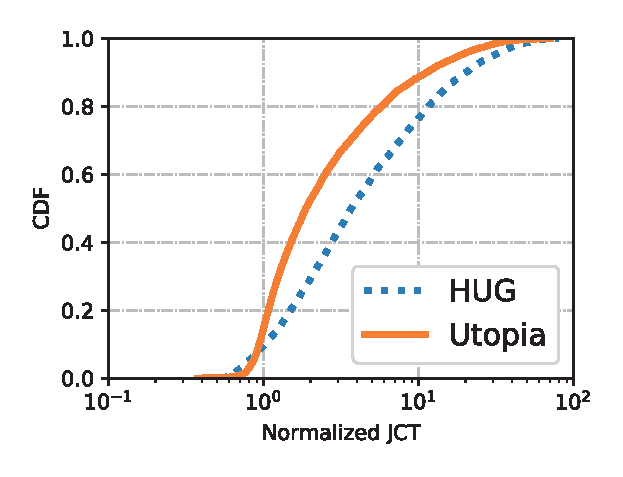
\includegraphics[width=0.5\linewidth]{isolation1.eps}\label{f1:1}}
	\hfil
	\subfloat[Average normalized JCT]{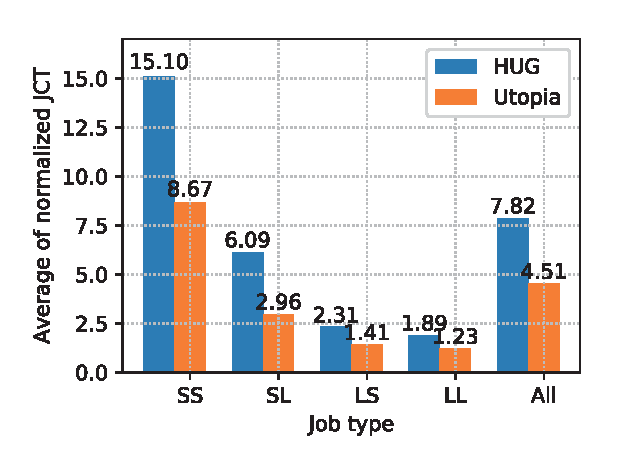
\includegraphics[width=0.5\linewidth]{isolation2.eps}\label{f1:2}}
	\caption{Characteristics of long-term isolation guarantee. (a) Distribution of normalized JCT. (b) Average normalized JCT of different job types.}
	\label{f1}
\end{figure}

For better understanding of the performance impact on different jobs, we further divide all jobs into four bins based on their total size and number of dependencies. Specifically, we consider a job \emph{small} (\emph{large}) if its total size is less (more) than half of jobs in specific time of simulation, and \emph{short} (\emph{long}) if it contains less (more) dependencies than $\beta/2$ where $\beta$ is the average number of coflows in a job.

The average normalized JCTs of the two baseline schedulers in four different types are compared as shown in Fig.~\ref{f1}(b). A general trend can be observed that the normalized JCT of a \emph{small} (\emph{short}) job is much likely higher than that of a \emph{large} (\emph{long}) job. This trend is reasonable for our algorithm based on a completion time order specified by a fair scheduler. Because of the dominance of small jobs (more than 70\% in our simulation), speeding up their completion significantly increases the average performance. On average, our scheduler can speed up a job's completion by 7.82$\times$ (4.51$\times$) in expectation compared with HUG (Utopia).

\subsection{Performance}
We next evaluate the performance (\emph{i.e.}, average JCT) of our scheduler with other baseline schedulers given different parameters ($\alpha$ and $\beta$). Because of small jobs are in the majority of all jobs (60\% of all), %In curious of how far all these schedulers are from optimal,
we define a new metric called average \emph{job slowdown} instead of average JCT in our evaluation by borrowing the idea from \emph{coflow slowdown} defined in \cite{utopia}. Job slowdown is defined as
\[\text{Job slowdown} = \frac{\text{Compared JCT}}{\text{Minimum JCT if running alone}}.\]
As shown in Fig.~\ref{f2}(a), the JCT of our scheduler is much smaller than those of the three baseline schedulers overall. We next discuss the influence of the two parameters $\alpha$ and $\beta$.

\begin{figure*}[!t]
	\centering
	\subfloat[CDF of job slowdown]{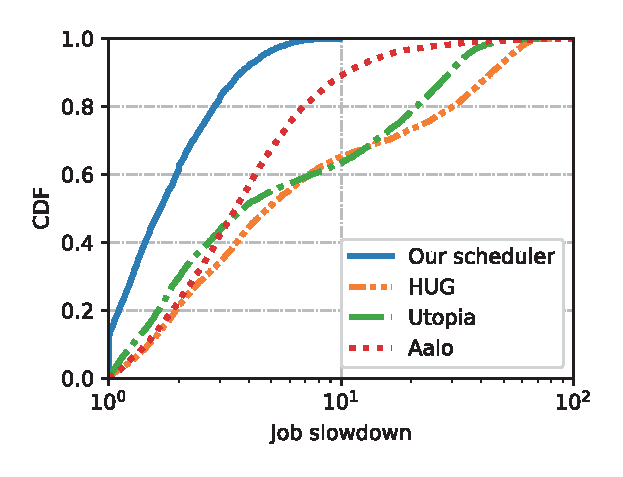
\includegraphics[width=0.333\linewidth]{performance3.eps}\label{f2:3}}
	\hfil
	\subfloat[The \# of machines ($\alpha$)]{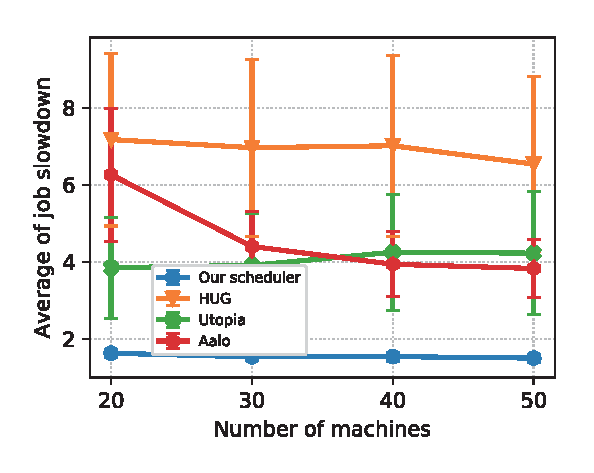
\includegraphics[width=0.32\linewidth]{performance1.eps}\label{f2:1}}
	\hfil
	\subfloat[Average \# of coflows in each job ($\beta$)]{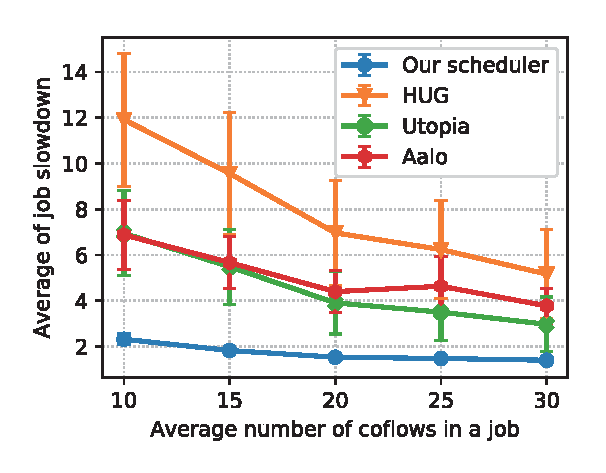
\includegraphics[width=0.33\linewidth]{performance2.eps}\label{f2:2}}
	\caption{Characteristics of performance. (a) CDF of job slowdown. (b) Average job slowdown in different number of machines. (c) Average job slowdown in different average number of coflows in each job.}
	\label{f2}
\end{figure*}

First, we investigate the influence of $\alpha$, \emph{i.e.}, the number of machines, as shown in Fig.~\ref{f2}(b). As discussed in Section~\ref{evaluation}, the total bandwidth grows linearly as $\alpha$ increases. However, the average job slowdown does not increase in reciprocal proportion of $\alpha$ because of the non-uniformity of coflow space distribution. Compared with HUG, Utopia, and Aalo, we reduce the average slowdown by up to 92\%, 88\%, and 90\%, respectively.

Second, we investigate the influence of $\beta$, \emph{i.e.}, the average number of coflows in each job, as shown in Fig.~\ref{f2}(c). We can see that all four lines decrease with similar gradient. Compared with HUG, Utopia, and Aalo, we reduce the average slowdown by up to 92\%, 86\%, and 89\%, respectively.

Overall, our scheduler outperforms baseline schedulers significantly. We believe the main reason is that baseline schedulers focus on the coflow-level scheduling while ours focuses on job-level scheduling.

\section{Conclusion}
In this paper, a coflow scheduler of multi-stage jobs is proposed. To the best of our knowledge, our work is the first coflow scheduler that aims to simultaneously minimize the average JCT and serve isolation guarantee in the context of multi-stage jobs. We prove that our scheduler can provide long-term isolation guarantee. The trace-driven evaluations have confirmed that our scheduler achieves near-optimal performance compared with the state-of-the-art schedulers.

\section*{Acknowledgment}
This work is supported in part by the National Science Foundation of China under Grants (No. 61672276, No. 61502229, No. 61872178), the National Key Research and Development Program of China under Grant (No. 2017YFB1400601), the Fundamental Research Funds for the Central Universities (No. 021014380079), and the Collaborative Innovation Center of Novel Software Technology and Industrialization, Nanjing University.

\bibliographystyle{IEEEtran}
\bibliography{IEEEfull,myref}

%\begin{thebibliography}{00}
%\bibitem{b1} G. Eason, B. Noble, and I. N. Sneddon, ``On certain integrals of Lipschitz-Hankel type involving products of Bessel functions,'' Phil. Trans. Roy. Soc. London, vol. A247, pp. 529--551, April 1955.
%\bibitem{b2} J. Clerk Maxwell, A Treatise on Electricity and Magnetism, 3rd ed., vol. 2. Oxford: Clarendon, 1892, pp.68--73.
%\bibitem{b3} I. S. Jacobs and C. P. Bean, ``Fine particles, thin films and exchange anisotropy,'' in Magnetism, vol. III, G. T. Rado and H. Suhl, Eds. New York: Academic, 1963, pp. 271--350.
%\bibitem{b4} K. Elissa, ``Title of paper if known,'' unpublished.
%\bibitem{b5} R. Nicole, ``Title of paper with only first word capitalized,'' J. Name Stand. Abbrev., in press.
%\bibitem{b6} Y. Yorozu, M. Hirano, K. Oka, and Y. Tagawa, ``Electron spectroscopy studies on magneto-optical media and plastic substrate interface,'' IEEE Transl. J. Magn. Japan, vol. 2, pp. 740--741, August 1987 [Digests 9th Annual Conf. Magnetics Japan, p. 301, 1982].
%\bibitem{b7} M. Young, The Technical Writer's Handbook. Mill Valley, CA: University Science, 1989.
%\end{thebibliography}
%\vspace{12pt}
%\color{red}
%IEEE conference templates contain guidance text for composing and formatting conference papers. Please ensure that all template text is removed from your conference paper prior to submission to the conference. Failure to remove the template text from your paper may result in your paper not being published.

\end{document}
